\documentclass[11pt]{article}

\usepackage[margin=2.5cm]{geometry}
\usepackage{amsmath,amssymb,amsthm,mathtools}
\usepackage{booktabs}
\usepackage{xcolor}
\usepackage{tikz}
\usetikzlibrary{patterns,positioning,decorations.pathreplacing}
\usepackage{algorithm}
\usepackage{algpseudocode}
\usepackage{hyperref}
\hypersetup{colorlinks=true,linkcolor=blue!50!black,citecolor=blue!50!black,urlcolor=blue!50!black}

% ---------------------------------------------------------------------------
% Notation
\newcommand{\ct}{^{\mathsf H}}            % conjugate transpose
\newcommand{\hU}{\widehat U}
\newcommand{\hV}{\widehat V}
\newcommand{\cV}{\breve V}
\newcommand{\hQ}{\widehat Q}
\newcommand{\hD}{\widehat D}
\newcommand{\hx}{\hat x}
\newcommand{\hb}{\hat b}
\newcommand{\htau}{\hat\tau}

\theoremstyle{definition}
\newtheorem{remark}{Remark}
\newtheorem{observation}{Key observation}

% Colours used in the block pictures
\colorlet{nz}{blue!25}      % generic nonzero block
\colorlet{tri}{red!55}      % triangular block that is solved
\colorlet{gone}{gray!12}    % rows/columns that have been eliminated

\title{The implicit ULV elimination for SSS and HSS matrices\\[2pt]
\large A worked $4\times4$ walk-through}
\author{}
\date{}

\begin{document}
\maketitle

\begin{abstract}
These notes explain, step by step, the fast backward-stable solvers of
Chandrasekaran, Dewilde, Gu, Pals and van der Veen for sequentially
semi-separable (SSS) matrices~\cite{CDGPV02,CDGPSVW05} and of Chandrasekaran,
Gu and Pals for hierarchically semi-separable (HSS) matrices~\cite{CGP06}.
Both solvers compute a factorization $A = \mathcal U\,\mathcal L\,\mathcal V$
with $\mathcal U,\mathcal V$ unitary and $\mathcal L$ (block) lower triangular,
without ever forming the three factors; this is what is meant by an
\emph{implicit ULV decomposition}. We use the same $4\times4$ block example
throughout so that the two algorithms can be compared line by line.
\end{abstract}

\tableofcontents

% ===========================================================================
\section*{The one idea behind both algorithms}
\addcontentsline{toc}{section}{The one idea behind both algorithms}

Consider one block row of a linear system $Ax=b$, say with $m$ rows. Split it
into its diagonal block $D$ and everything else (the off-diagonal part). In a
rank-structured matrix the off-diagonal part of that block row has the form
$U\,(\text{something})$, where $U$ has $m$ rows but only $k<m$ columns. The
column space of the off-diagonal part is therefore at most $k$-dimensional,
which means that there are $m-k$ independent combinations of the $m$ equations
in which the off-diagonal part cancels completely. Those $m-k$ combined
equations only involve the unknowns of the diagonal block.

The solvers exploit this in three moves, applied over and over:

\begin{enumerate}
  \item \textbf{Compress (from the left).} Find a unitary $q$ with
    $q\ct U = \left(\begin{smallmatrix}0\\ \hU\end{smallmatrix}\right)$. After multiplying
    the block row by $q\ct$, its first $m-k$ rows are zero outside the diagonal block.
  \item \textbf{Triangularize (from the right).} Those $m-k$ rows still couple to all
    $m$ unknowns of the diagonal block. Find a unitary $w$ such that
    $(q\ct D)\,w\ct$ is lower triangular, and change variables to $w x$. Now the
    first $m-k$ equations involve only the first $m-k$ new unknowns, which form
    a small triangular system.
  \item \textbf{Solve, update, deflate.} Solve the small triangular system,
    move its contribution to the right-hand side, and delete those rows and columns.
    What is left is a smaller system \emph{with the same rank structure}, so the
    procedure can be repeated.
\end{enumerate}

When no block row can be compressed any more (because $k\geq m$), neighbouring
blocks are \textbf{merged} into a bigger block. This makes the diagonal block larger
while the rank $k$ of its off-diagonal part stays small, so compression becomes
possible again.

Only unitary transformations and small triangular solves are used, which is
why the solvers are backward stable. Because the transformations are applied
on the fly and never stored as big matrices, the ULV factorization stays
implicit.

SSS and HSS differ only in \emph{which} blocks are compressed when, and in
\emph{how} the solved unknowns are propagated to the remaining equations.

% ===========================================================================
\section{SSS matrices: eliminating one block row at a time}
\label{sec:sss}

\subsection{\texorpdfstring{The $4\times4$ SSS matrix}{The 4x4 SSS matrix}}

We use the notation of~\cite[Section~5]{CDGPV02}. Let the unknown $x$ and the
right-hand side $b$ be partitioned into four blocks of sizes $m_1,\dots,m_4$.
A $4\times4$ SSS matrix is
\begin{equation}
\label{eq:sss}
A =
\begin{pmatrix}
D_1 & U_1V_2\ct & U_1W_2V_3\ct & U_1W_2W_3V_4\ct \\[2pt]
P_2Q_1\ct & D_2 & U_2V_3\ct & U_2W_3V_4\ct \\[2pt]
P_3R_2Q_1\ct & P_3Q_2\ct & D_3 & U_3V_4\ct \\[2pt]
P_4R_3R_2Q_1\ct & P_4R_3Q_2\ct & P_4Q_3\ct & D_4
\end{pmatrix}.
\end{equation}
The pattern is easy to read off:
\begin{itemize}
  \item block $(i,j)$ with $i<j$ (upper part) is $U_i\,W_{i+1}\cdots W_{j-1}\,V_j\ct$;
  \item block $(i,j)$ with $i>j$ (lower part) is $P_i\,R_{i-1}\cdots R_{j+1}\,Q_j\ct$.
\end{itemize}
Two facts drive everything that follows.
\begin{observation}
\label{obs:sss-row}
Every block in the strictly upper part of block row $i$ starts with $U_i$.
Every block in the strictly lower part of block column $j$ ends with $Q_j\ct$.
\end{observation}
We write $k_i$ for the number of columns of $U_i$. The dimension that decides
what the algorithm does at block~1 is $k_1$ compared with $m_1$.

\paragraph{An extra term on the right-hand side.}
The algorithm is recursive, and to make every recursive call look the same we
solve the slightly more general system
\begin{equation}
\label{eq:sss-system}
A\,x \;=\; b \;-\;
\begin{pmatrix} 0\\ P_2\\ P_3R_2\\ P_4R_3R_2 \end{pmatrix}\tau ,
\end{equation}
with $\tau=0$ at the start. Compare the coefficient of $\tau$ with the first
block column of~\eqref{eq:sss}. It is exactly the strictly lower part of that
column with the trailing $Q_1\ct$ removed. So $\tau$ behaves like an extra
unknown in a ``block column~0'' to the left of the matrix whose value is
already known. Its role is to carry the influence of unknowns that have
already been eliminated down to the rows that have not yet been processed. In
system-theory language, $\tau$ is the \emph{state} of the lower (causal) part of
the matrix.

\subsection{\texorpdfstring{Case $k_1<m_1$: elimination}{Case k1 < m1: elimination}}

\subsubsection*{Step 1: compress block row 1 from the left}

By Key observation~\ref{obs:sss-row}, the whole strictly upper part of block row 1 equals
\[
U_1\,\bigl(\,V_2\ct \;\; W_2V_3\ct \;\; W_2W_3V_4\ct\,\bigr).
\]
Its column space lies inside the column space of $U_1$, which has dimension at
most $k_1<m_1$. Compute a QL factorization of the tall matrix $U_1$:
\[
U_1 = q_1\begin{pmatrix}0\\ \hU_1\end{pmatrix}
\begin{matrix}\}\,m_1-k_1\\ \}\,k_1\phantom{-m_1}\end{matrix},
\qquad\text{i.e.}\qquad
q_1\ct U_1 = \begin{pmatrix}0\\ \hU_1\end{pmatrix},
\]
with $q_1$ an $m_1\times m_1$ unitary matrix. Multiply the first block row of
the equations by $q_1\ct$. Only three things change:
\begin{itemize}
  \item $U_1 \to \left(\begin{smallmatrix}0\\ \hU_1\end{smallmatrix}\right)$, so every upper block in row 1
    now has $m_1-k_1$ zero rows on top;
  \item $D_1\to q_1\ct D_1$;
  \item $b_1\to q_1\ct b_1 = \left(\begin{smallmatrix}\beta_1\\ \gamma_1\end{smallmatrix}\right)$,
    split into $m_1-k_1$ and $k_1$ rows.
\end{itemize}
The $\tau$ term does not change, because its first block is $0$. The lower
blocks in rows $2,3,4$ do not change either, because we only touched row 1.

\subsubsection*{Step 2: triangularize the diagonal block from the right}

The top $m_1-k_1$ rows of block row 1 are now zero \emph{except} in the
diagonal block, where they are the dense $(m_1-k_1)\times m_1$ matrix formed by the top rows of
$q_1\ct D_1$. To isolate a square subsystem we compute an LQ factorization:
\[
(q_1\ct D_1)\,w_1\ct =
\begin{pmatrix}
D_{11} & 0\\
D_{21} & D_{22}
\end{pmatrix}
\begin{matrix}\}\,m_1-k_1\\ \}\,k_1\phantom{-m_1}\end{matrix},
\qquad D_{11}\ \text{lower triangular},
\]
with $w_1$ unitary. Multiply block column 1 by $w_1\ct$ from the right. To keep the equations
unchanged we have to change variables accordingly:
\[
A x = (A\,\mathrm{diag}(w_1\ct,I,I,I))\,(\mathrm{diag}(w_1,I,I,I)\,x),
\qquad
w_1x_1 = \begin{pmatrix} z_1\\ \hx_1\end{pmatrix}
\begin{matrix}\}\,m_1-k_1\\ \}\,k_1\phantom{-m_1}\end{matrix}.
\]
By Key observation~\ref{obs:sss-row}, every lower block in column~1 ends with $Q_1\ct$, so it
becomes $\cdots Q_1\ct w_1\ct = \cdots (w_1Q_1)\ct$. Split
\[
w_1Q_1 = \begin{pmatrix} Q_{11}\\ \hQ_1\end{pmatrix}
\begin{matrix}\}\,m_1-k_1\\ \}\,k_1\phantom{-m_1}\end{matrix}.
\]
After both transformations the system reads (block sizes are
$m_1-k_1,\,k_1,\,m_2,\,m_3,\,m_4$):
\begin{equation}
\label{eq:sss-after}
\begin{pmatrix}
\color{red!70!black}D_{11} & 0 & 0 & 0 & 0\\[2pt]
D_{21} & D_{22} & \hU_1V_2\ct & \hU_1W_2V_3\ct & \hU_1W_2W_3V_4\ct\\[2pt]
P_2Q_{11}\ct & P_2\hQ_1\ct & D_2 & U_2V_3\ct & U_2W_3V_4\ct\\[2pt]
P_3R_2Q_{11}\ct & P_3R_2\hQ_1\ct & P_3Q_2\ct & D_3 & U_3V_4\ct\\[2pt]
P_4R_3R_2Q_{11}\ct & P_4R_3R_2\hQ_1\ct & P_4R_3Q_2\ct & P_4Q_3\ct & D_4
\end{pmatrix}
\begin{pmatrix} z_1\\ \hx_1\\ x_2\\ x_3\\ x_4\end{pmatrix}
=
\begin{pmatrix} \beta_1\\ \gamma_1\\ b_2\\ b_3\\ b_4\end{pmatrix}
-
\begin{pmatrix} 0\\ 0\\ P_2\\ P_3R_2\\ P_4R_3R_2\end{pmatrix}\tau .
\end{equation}

\subsubsection*{Step 3: solve the triangular system}

The first block equation in~\eqref{eq:sss-after} now involves only $z_1$:
\[
D_{11}\,z_1 = \beta_1 .
\]
This is a small lower-triangular system, solved by forward substitution. It is
the ``L'' in ULV.

\subsubsection*{\texorpdfstring{Step 4: push $z_1$ to the right-hand side}{Step 4: push z1 to the right-hand side}}

The rest of column $z_1$ in~\eqref{eq:sss-after} has to be moved to the right-hand side:
\begin{itemize}
  \item In the $\gamma_1$ row: $\hb_1 := \gamma_1 - D_{21}z_1$.
  \item In rows $2,3,4$: the coefficient of $z_1$ is
    $\left(\begin{smallmatrix}P_2\\P_3R_2\\P_4R_3R_2\end{smallmatrix}\right)Q_{11}\ct$.
    This is the \emph{same} column of generators that multiplies $\tau$. So the update costs
    nothing more than
    \[
    \htau := \tau + Q_{11}\ct z_1 .
    \]
\end{itemize}
The second bullet is the elegant part of the SSS algorithm. The effect of $z_1$ on all
later rows is summarized by a vector $\htau$ of small size. We never touch rows $2,3,4$.

\subsubsection*{Step 5: deflate and recurse}

Drop the first $m_1-k_1$ rows and columns. What remains is
\[
\begin{pmatrix}
D_{22} & \hU_1V_2\ct & \hU_1W_2V_3\ct & \hU_1W_2W_3V_4\ct\\[2pt]
P_2\hQ_1\ct & D_2 & U_2V_3\ct & U_2W_3V_4\ct\\[2pt]
P_3R_2\hQ_1\ct & P_3Q_2\ct & D_3 & U_3V_4\ct\\[2pt]
P_4R_3R_2\hQ_1\ct & P_4R_3Q_2\ct & P_4Q_3\ct & D_4
\end{pmatrix}
\begin{pmatrix} \hx_1\\ x_2\\ x_3\\ x_4\end{pmatrix}
=
\begin{pmatrix} \hb_1\\ b_2\\ b_3\\ b_4\end{pmatrix}
-
\begin{pmatrix} 0\\ P_2\\ P_3R_2\\ P_4R_3R_2\end{pmatrix}\htau ,
\]
which is again of the form~\eqref{eq:sss-system}. Only the first block has
changed, and it has shrunk from $m_1$ to $k_1$ rows and columns. The update of
the representation is
\[
\begin{array}{c|c|c|c|c|c}
\text{quantity} & D_1 & U_1 & Q_1 & b_1 & \tau\\\hline
\text{becomes} & D_{22} & \hU_1 & \hQ_1 & \hb_1=\gamma_1-D_{21}z_1 & \htau=\tau+Q_{11}\ct z_1
\end{array}
\]
and every other generator is untouched. Once the smaller system has been
solved (recursively) for $\hx_1, x_2, x_3, x_4$, the original first block is recovered by
\[
x_1 = w_1\ct\begin{pmatrix} z_1\\ \hx_1\end{pmatrix}.
\]

Figure~\ref{fig:sss} shows the sparsity pattern during these five steps.

\begin{figure}[t]
\centering
% helper macros for 4x4 block pictures (unit blocks, row i at y in [-i,-i+1])
\newcommand{\fillblock}[3]{\fill[#3] (#2-1,-#1) rectangle (#2,-#1+1);}
\newcommand{\topstrip}[3]{\fill[#3] (#2-1,-#1+0.5) rectangle (#2,-#1+1);}
\newcommand{\leftstrip}[3]{\fill[#3] (#2-1,-#1) rectangle (#2-0.5,-#1+1);}
\newcommand{\topright}[3]{\fill[#3] (#2-0.5,-#1+0.5) rectangle (#2,-#1+1);}
\newcommand{\toplefttri}[3]{\fill[white] (#2-1,-#1+0.5) rectangle (#2-0.5,-#1+1);
  \fill[#3] (#2-1,-#1+1) -- (#2-1,-#1+0.5) -- (#2-0.5,-#1+0.5) -- cycle;}
\newcommand{\grid}{\draw[thick] (0,-4) rectangle (4,0);
  \foreach \k in {1,2,3}{\draw (\k,0) -- (\k,-4); \draw (0,-\k) -- (4,-\k);}}
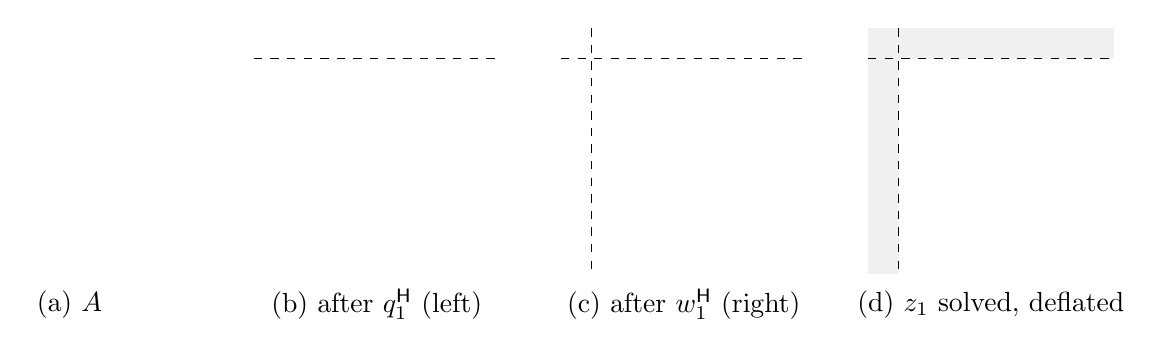
\begin{tikzpicture}[scale=0.78]
  % (a) original
  \begin{scope}
    \foreach \i in {1,...,4}{\foreach \j in {1,...,4}{\fillblock{\i}{\j}{nz}}}
    \grid
    \node at (2,-4.5) {(a) $A$};
  \end{scope}
  % (b) after q_1^H
  \begin{scope}[xshift=5cm]
    \foreach \i in {1,...,4}{\foreach \j in {1,...,4}{\fillblock{\i}{\j}{nz}}}
    \foreach \j in {2,3,4}{\topstrip{1}{\j}{white}}
    \grid \draw[dashed] (0,-0.5) -- (4,-0.5);
    \node at (2,-4.5) {(b) after $q_1\ct$ (left)};
  \end{scope}
  % (c) after w_1^H
  \begin{scope}[xshift=10cm]
    \foreach \i in {1,...,4}{\foreach \j in {1,...,4}{\fillblock{\i}{\j}{nz}}}
    \foreach \j in {2,3,4}{\topstrip{1}{\j}{white}}
    \topright{1}{1}{white} \toplefttri{1}{1}{tri}
    \grid \draw[dashed] (0,-0.5) -- (4,-0.5); \draw[dashed] (0.5,0) -- (0.5,-4);
    \node at (2,-4.5) {(c) after $w_1\ct$ (right)};
  \end{scope}
  % (d) deflated
  \begin{scope}[xshift=15cm]
    \foreach \i in {1,...,4}{\foreach \j in {1,...,4}{\fillblock{\i}{\j}{nz}}}
    \fill[gone] (0,0) rectangle (4,-0.5);
    \fill[gone] (0,0) rectangle (0.5,-4);
    \grid \draw[dashed] (0,-0.5) -- (4,-0.5); \draw[dashed] (0.5,0) -- (0.5,-4);
    \node at (2,-4.5) {(d) $z_1$ solved, deflated};
  \end{scope}
\end{tikzpicture}
\caption{One elimination step on block 1 of a $4\times4$ SSS matrix. Blue: nonzero;
white: zero; red: the lower-triangular $D_{11}$ that is solved for $z_1$; grey:
rows and columns removed after $z_1$ is known. The contribution of the grey
column to block rows $2$--$4$ is absorbed into $\tau$.}
\label{fig:sss}
\end{figure}

\subsection{\texorpdfstring{Case $k_1\geq m_1$: merge}{Case k1 >= m1: merge}}

If $U_1$ has at least as many columns as rows, a transformation from the left
cannot create zero rows, so there is nothing to compress. Instead we merge the
first two block rows and columns into one block. Rewriting~\eqref{eq:sss-system} with the
$2\times2$ leading block grouped gives
\[
\left(
\begin{array}{c|cc}
\begin{pmatrix} D_1 & U_1V_2\ct\\ P_2Q_1\ct & D_2\end{pmatrix} &
\begin{pmatrix} U_1W_2\\ U_2\end{pmatrix}V_3\ct &
\begin{pmatrix} U_1W_2\\ U_2\end{pmatrix}W_3V_4\ct\\[10pt]\hline
P_3\begin{pmatrix} Q_1R_2\ct\\ Q_2\end{pmatrix}\ct & D_3 & U_3V_4\ct\\[10pt]
P_4R_3\begin{pmatrix} Q_1R_2\ct\\ Q_2\end{pmatrix}\ct & P_4Q_3\ct & D_4
\end{array}
\right)
\begin{pmatrix} \begin{pmatrix}x_1\\x_2\end{pmatrix}\\ x_3\\ x_4\end{pmatrix}
\]
\[
\qquad\qquad=
\begin{pmatrix} \begin{pmatrix}b_1\\ b_2-P_2\tau\end{pmatrix}\\ b_3\\ b_4\end{pmatrix}
-
\begin{pmatrix} 0\\ P_3\\ P_4R_3\end{pmatrix}(R_2\tau).
\]
This is a $3\times3$ SSS system of the form~\eqref{eq:sss-system} with
\[
\hD_1=\begin{pmatrix} D_1 & U_1V_2\ct\\ P_2Q_1\ct & D_2\end{pmatrix},\quad
\hU_1=\begin{pmatrix} U_1W_2\\ U_2\end{pmatrix},\quad
\hQ_1=\begin{pmatrix} Q_1R_2\ct\\ Q_2\end{pmatrix},\quad
\hb_1=\begin{pmatrix} b_1\\ b_2-P_2\tau\end{pmatrix},\quad
\htau = R_2\tau .
\]
No arithmetic is done on the matrix itself; the merge only regroups the
generators (the products $U_1W_2$, $Q_1R_2\ct$ and $R_2\tau$ are small).
After the merge the first block has $m_1+m_2$ rows, but $\hU_1$ has only
$k_2$ columns, so it will typically be compressible at the next step.

\subsection{Putting it together: the rhythm of the algorithm}

\begin{algorithm}[h]
\caption{Implicit ULV solve of an SSS system~\eqref{eq:sss-system} (after~\cite[Section~5.2]{CDGPV02})}
\label{alg:sss}
\begin{algorithmic}[1]
\Function{SSS-Solve}{$\{D_i,U_i,V_i,W_i,P_i,Q_i,R_i\}_{i=1}^n,\ b,\ \tau$}
\If{$n=1$} \State \Return $x_1 = D_1^{-1} b_1$ \Comment{dense solve, e.g.\ via QR}
\ElsIf{$k_1<m_1$} \Comment{elimination}
  \State QL: $q_1\ct U_1 = \left(\begin{smallmatrix}0\\ \hU_1\end{smallmatrix}\right)$;\quad
         $\left(\begin{smallmatrix}\beta_1\\ \gamma_1\end{smallmatrix}\right)= q_1\ct b_1$
  \State LQ: $(q_1\ct D_1)w_1\ct = \left(\begin{smallmatrix}D_{11}&0\\ D_{21}&D_{22}\end{smallmatrix}\right)$;\quad
         $\left(\begin{smallmatrix}Q_{11}\\ \hQ_1\end{smallmatrix}\right)= w_1Q_1$
  \State $z_1 = D_{11}^{-1}\beta_1$ \Comment{triangular solve}
  \State $\hb_1 = \gamma_1-D_{21}z_1$;\quad $\htau = \tau + Q_{11}\ct z_1$
  \State $(\hx_1,x_2,\dots,x_n) = $ \Call{SSS-Solve}{generators with $D_1,U_1,Q_1\to D_{22},\hU_1,\hQ_1$;\ $b_1\to\hb_1$;\ $\htau$}
  \State \Return $x_1 = w_1\ct\left(\begin{smallmatrix}z_1\\ \hx_1\end{smallmatrix}\right),\ x_2,\dots,x_n$
\Else \Comment{merge blocks 1 and 2}
  \State form $\hD_1,\hU_1,\hQ_1,\hb_1,\htau$ as in the merge formulas
  \State $(\hx_1,x_3,\dots,x_n) = $ \Call{SSS-Solve}{$n-1$ blocks with the merged first block, $\htau$}
  \State \Return $(x_1,x_2) = \hx_1$ split, $x_3,\dots,x_n$
\EndIf
\EndFunction
\end{algorithmic}
\end{algorithm}

On the $4\times4$ example, with every $k_i<m_i$, the recursion goes
\begin{gather*}
\underbrace{\text{eliminate in }1}_{m_1\to k_1}
\;\to\;
\underbrace{\text{merge }1,2}_{\text{size } k_1+m_2}
\;\to\;
\text{eliminate}
\;\to\;
\text{merge with }3\\
\;\to\;
\text{eliminate}
\;\to\;
\text{merge with }4
\;\to\;
\text{eliminate}
\;\to\;
\text{dense solve } (n=1).
\end{gather*}
Elimination and merging always alternate. After an elimination the first
block has exactly $k_1$ rows, which equals the number of columns of $\hU_1$, so
it cannot be compressed again until it is merged with the next block. The
algorithm is a single top-to-bottom sweep, followed by a bottom-to-top sweep
that applies the stored $w_i\ct$ to recover $x$. With block sizes and ranks
bounded, the total work is $O(N)$.

\subsection{Why this is a ULV decomposition}
\label{sec:sss-ulv}

Collect all the left transformations ($q_1\ct$ and the later ones, each embedded
in an identity) into one unitary matrix $\mathcal U\ct$, and all the right
transformations into $\mathcal V\ct$. Order the unknowns in the order in
which they are solved: $z^{(1)}, z^{(2)},\dots$, and finally the unknowns of the
last dense solve. Order the equations the same way. Then:
\begin{itemize}
  \item the equation block that determines $z^{(s)}$ contains only $z^{(s)}$
    (through a triangular $D_{11}$) and the earlier $z^{(1)},\dots,z^{(s-1)}$, whose contributions
    were moved to the right-hand side. All later unknowns have zero coefficients,
    because the corresponding rows were zeroed by compression;
  \item merges only regroup blocks and introduce no new factors.
\end{itemize}
Hence, for a permutation $\Pi$ that encodes this elimination order,
\[
\Pi^{\mathsf T}\bigl(\mathcal U\ct A\,\mathcal V\ct\bigr)\Pi = \mathcal L
\quad\Longrightarrow\quad
A = (\mathcal U\Pi)\,\mathcal L\,(\Pi^{\mathsf T}\mathcal V),
\]
with $\mathcal L$ block lower triangular, whose diagonal blocks are the triangular
$D_{11}$'s (plus the final dense block, which an LQ factorization also makes triangular).
The algorithm never forms $\mathcal U$, $\mathcal L$ or $\mathcal V$. It applies
them to $b$ one small piece at a time, which is why the decomposition is called implicit.

% ===========================================================================
\section{HSS matrices: eliminating all leaves at once}
\label{sec:hss}

We now follow~\cite[Section~4]{CGP06}. The paper states the main
difference itself: \emph{``The basic idea of the algorithm is akin to that for the SSS
representation. The one major difference is that we operate on all block rows at
the same time.''}

\subsection{\texorpdfstring{The $4\times4$ HSS matrix}{The 4x4 HSS matrix}}

Take a two-level binary tree with leaves $1,2,3,4$, parents $\alpha=\{1,2\}$
and $\beta=\{3,4\}$, and the root $\{1,2,3,4\}$ (Figure~\ref{fig:tree}). To keep
the formulas short we drop the level index of~\cite{CGP06}:
\begin{gather*}
D_i \equiv D_{2;i},\quad U_i\equiv U_{2;i},\quad V_i\equiv V_{2;i},\quad
R_i\equiv R_{2;i},\quad W_i\equiv W_{2;i},\\
B_{12}\equiv B_{2;1,2},\ \dots,\ B_{43}\equiv B_{2;4,3},\qquad B_{\alpha\beta}\equiv B_{1;1,2},\quad B_{\beta\alpha}\equiv B_{1;2,1}.
\end{gather*}
The bases of the parents are not stored. They are generated from the
children by the translation operators $R_i, W_i$:
\begin{equation}
\label{eq:nested}
U_\alpha = \begin{pmatrix} U_1R_1\\ U_2R_2\end{pmatrix},\quad
V_\alpha = \begin{pmatrix} V_1W_1\\ V_2W_2\end{pmatrix},\quad
U_\beta = \begin{pmatrix} U_3R_3\\ U_4R_4\end{pmatrix},\quad
V_\beta = \begin{pmatrix} V_3W_3\\ V_4W_4\end{pmatrix}.
\end{equation}
The matrix is
\[
A=\begin{pmatrix}
\begin{pmatrix} D_1 & U_1B_{12}V_2\ct\\ U_2B_{21}V_1\ct & D_2\end{pmatrix} &
U_\alpha B_{\alpha\beta}V_\beta\ct\\[12pt]
U_\beta B_{\beta\alpha}V_\alpha\ct &
\begin{pmatrix} D_3 & U_3B_{34}V_4\ct\\ U_4B_{43}V_3\ct & D_4\end{pmatrix}
\end{pmatrix},
\]
and written out block by block, using~\eqref{eq:nested},
\begin{equation}
\label{eq:hss}
A=
\begin{pmatrix}
D_1 & U_1B_{12}V_2\ct & U_1R_1B_{\alpha\beta}W_3\ct V_3\ct & U_1R_1B_{\alpha\beta}W_4\ct V_4\ct\\[2pt]
U_2B_{21}V_1\ct & D_2 & U_2R_2B_{\alpha\beta}W_3\ct V_3\ct & U_2R_2B_{\alpha\beta}W_4\ct V_4\ct\\[2pt]
U_3R_3B_{\beta\alpha}W_1\ct V_1\ct & U_3R_3B_{\beta\alpha}W_2\ct V_2\ct & D_3 & U_3B_{34}V_4\ct\\[2pt]
U_4R_4B_{\beta\alpha}W_1\ct V_1\ct & U_4R_4B_{\beta\alpha}W_2\ct V_2\ct & U_4B_{43}V_3\ct & D_4
\end{pmatrix}.
\end{equation}

\begin{figure}[!htb]
\centering
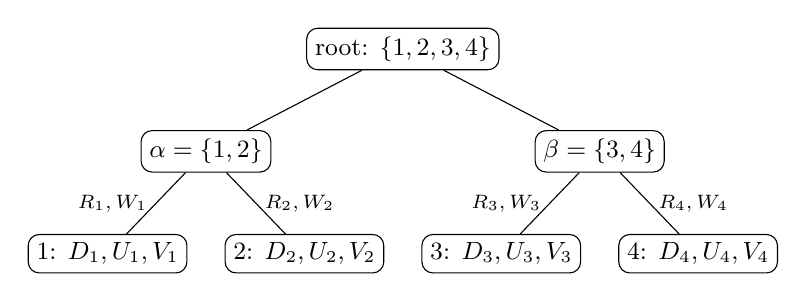
\begin{tikzpicture}[
  level distance=13mm,
  level 1/.style={sibling distance=50mm},
  level 2/.style={sibling distance=25mm},
  every node/.style={draw,rounded corners,inner sep=3pt,font=\small}]
\node {root: $\{1,2,3,4\}$}
  child { node {$\alpha=\{1,2\}$}
    child { node {$1$: $D_1,U_1,V_1$} edge from parent node[draw=none,left,font=\scriptsize] {$R_1,W_1$} }
    child { node {$2$: $D_2,U_2,V_2$} edge from parent node[draw=none,right,font=\scriptsize] {$R_2,W_2$} }
  }
  child { node {$\beta=\{3,4\}$}
    child { node {$3$: $D_3,U_3,V_3$} edge from parent node[draw=none,left,font=\scriptsize] {$R_3,W_3$} }
    child { node {$4$: $D_4,U_4,V_4$} edge from parent node[draw=none,right,font=\scriptsize] {$R_4,W_4$} }
  };
\end{tikzpicture}
\caption{The HSS tree of the $4\times4$ example. Siblings are coupled by
$B_{12},B_{21}$, $B_{34},B_{43}$ (leaf level) and $B_{\alpha\beta},B_{\beta\alpha}$ (level~1).}
\label{fig:tree}
\end{figure}

Key observation~\ref{obs:sss-row} carries over word for word, but now it holds for
\emph{every} block row and column at the same time:
\begin{observation}
\label{obs:hss}
In~\eqref{eq:hss}, every off-diagonal block in block row $i$ starts with $U_i$,
whether the block couples to the sibling ($U_iB\cdots$) or to the other half
of the tree ($U_iR_iB\cdots$). Every off-diagonal block in block column $j$ ends
with $V_j\ct$.
\end{observation}

In SSS this property holds only for the upper part of a block row, which is
why SSS starts at block~1 (it has no lower part) and proceeds sequentially. In
HSS it holds for the whole off-diagonal part of every block row, so all leaves
can be compressed simultaneously and independently.

Write $n_i$ for the number of columns of $U_i$ (the paper's $n_{K;i}$) and $m_i$
for the size of leaf $i$.

\subsection{\texorpdfstring{Case $n_i<m_i$: compressible off-diagonal blocks}{Case ni < mi: compressible off-diagonal blocks}}

\subsubsection*{Step 1: compress every block row (left)}

For each leaf $i=1,\dots,4$, independently, compute a QL factorization
\[
q_i\ct U_i = \begin{pmatrix} 0\\ \hU_i\end{pmatrix}
\begin{matrix}\}\,m_i-n_i\\ \}\,n_i\phantom{-m_i}\end{matrix},
\qquad
q_i\ct b_i = \begin{pmatrix} \beta_i\\ \gamma_i\end{pmatrix},
\]
and multiply block row $i$ by $q_i\ct$. By Key observation~\ref{obs:hss}, the top
$m_i-n_i$ rows of block row $i$ are now zero outside the diagonal block
(Figure~\ref{fig:hss}(a)). In matrix form we have multiplied by
$\mathrm{diag}(q_1\ct,q_2\ct,q_3\ct,q_4\ct)$ from the left.

\subsubsection*{Step 2: triangularize every diagonal block (right)}

For each $i$, compute an LQ factorization
\[
(q_i\ct D_i)\,w_i\ct = \begin{pmatrix} D_i^{11} & 0\\ D_i^{21} & D_i^{22}\end{pmatrix},
\]
and multiply block column $i$ by $w_i\ct$ from the right. By Key observation~\ref{obs:hss},
the only other change in column $i$ is $V_i\to w_iV_i$, which we split as
\[
w_iV_i = \begin{pmatrix} \cV_i\\ \hV_i\end{pmatrix}
\begin{matrix}\}\,m_i-n_i\\ \}\,n_i\phantom{-m_i}\end{matrix},
\qquad
w_ix_i = \begin{pmatrix} z_i\\ \hx_i\end{pmatrix}.
\]
This is Figure~\ref{fig:hss}(b). The transformed matrix
$\mathrm{diag}(q_i\ct)\,A\,\mathrm{diag}(w_i\ct)$ is again HSS. Its generators are
$\left(\begin{smallmatrix}D_i^{11}&0\\D_i^{21}&D_i^{22}\end{smallmatrix}\right)$,
$\left(\begin{smallmatrix}0\\\hU_i\end{smallmatrix}\right)$,
$\left(\begin{smallmatrix}\cV_i\\\hV_i\end{smallmatrix}\right)$, and the
\emph{unchanged} $R_i,W_i,B$'s.

\subsubsection*{Step 3: solve four triangular systems in parallel}

For each leaf $i$, the first $m_i-n_i$ equations read
\[
D_i^{11}z_i = \beta_i ,
\]
four small, independent lower-triangular solves. Unlike SSS, nothing has to
be done before these solves. All leaves are treated simultaneously, so this step
is naturally parallel.

\subsubsection*{\texorpdfstring{Step 4: push $z$ to the right-hand side}{Step 4: push z to the right-hand side}}

This is where HSS differs most from SSS. In SSS, $z_1$ belonged to the first
block, so it only affected rows below it, and its effect could be absorbed into
the single vector $\tau$. In HSS, $z_i$ affects \emph{every} other block row, both
above and below, through the column generators $\cV_i$.

Consider the remaining $n_i$ rows of block row $i$ (the $\gamma_i$ rows). For
$j\ne i$, their off-diagonal block in column $j$ has the form
\[
\hU_i\,(\cdots)\,\bigl(\cV_j\ct\ \ \hV_j\ct\bigr),
\]
where $(\cdots)$ is the chain of $B$, $R$ and $W$ factors that links leaf $j$ to
leaf $i$ in~\eqref{eq:hss}. The part that multiplies the known $z_j$ is
$\hU_i(\cdots)\cV_j\ct z_j$. So we need, for every $i$,
\[
\hb_i = \gamma_i - D_i^{21}z_i - \hU_i f_i,
\qquad
f_i = \sum_{j\ne i} (\text{translation chain from } j \text{ to } i)\,\cV_j\ct z_j .
\]
This is exactly an HSS matrix--vector product with the vector
$\bar z = \bigl(\begin{smallmatrix}z_i\\0\end{smallmatrix}\bigr)_{i=1}^4$, and it is computed
by the fast multiplication of~\cite[Section~3]{CGP06}, which has two passes:

\medskip
\noindent\textbf{Up-sweep} (leaves to root: compress what each subtree ``sends out''):
\[
g_i = \cV_i\ct z_i\ \ (i=1,\dots,4),\qquad
g_\alpha = W_1\ct g_1 + W_2\ct g_2,\qquad
g_\beta = W_3\ct g_3 + W_4\ct g_4 .
\]
\textbf{Down-sweep} (root to leaves: collect what each subtree ``receives''):
\[
f_\alpha = B_{\alpha\beta}\,g_\beta,\qquad f_\beta = B_{\beta\alpha}\,g_\alpha,
\]
\[
f_1 = B_{12}g_2 + R_1f_\alpha,\quad
f_2 = B_{21}g_1 + R_2f_\alpha,\quad
f_3 = B_{34}g_4 + R_3f_\beta,\quad
f_4 = B_{43}g_3 + R_4f_\beta .
\]
To check one entry, expand $\hU_1f_1$:
$\hU_1B_{12}\cV_2\ct z_2 + \hU_1R_1B_{\alpha\beta}(W_3\ct\cV_3\ct z_3 + W_4\ct\cV_4\ct z_4)$.
These are exactly the $z$-parts of the off-diagonal blocks $(1,2),(1,3),(1,4)$
in~\eqref{eq:hss} after the transformations.

\begin{remark}[$\tau$ versus $f$]
The SSS state $\tau$ and the HSS down-sweep vectors $f_i$ play the same role.
Both are short vectors that summarize the effect of all eliminated unknowns
on a block row. In SSS the information flows in one direction along a line,
so one running vector $\tau$ suffices and the update is $O(1)$ per step. In HSS
the information flows along a tree in both directions, so one up-sweep and one
down-sweep over the current tree are needed. Since the tree loses a level
after every round, the sweeps cost $O(N)$ in total.
\end{remark}

\subsubsection*{Step 5: deflate}

Drop the $z_i$ rows and columns of every leaf
(Figure~\ref{fig:hss}(c)). The remaining system
$\widehat A\,\hx = \hb$ has the HSS representation
\[
\{D_i^{22}\},\ \{\hU_i\},\ \{\hV_i\},\ \text{and the same } R_i,W_i,B_{12},B_{21},B_{34},B_{43},B_{\alpha\beta},B_{\beta\alpha}.
\]
Every leaf has shrunk from $m_i$ to $n_i$, and the tree is unchanged.
After this step every leaf has exactly as many rows ($n_i$) as $\hU_i$ has
columns, so no leaf can be compressed further. This is the same alternation
we saw in SSS.

\begin{figure}[t]
\centering
\newcommand{\fillblock}[3]{\fill[#3] (#2-1,-#1) rectangle (#2,-#1+1);}
\newcommand{\topstrip}[3]{\fill[#3] (#2-1,-#1+0.5) rectangle (#2,-#1+1);}
\newcommand{\topright}[3]{\fill[#3] (#2-0.5,-#1+0.5) rectangle (#2,-#1+1);}
\newcommand{\toplefttri}[3]{\fill[white] (#2-1,-#1+0.5) rectangle (#2-0.5,-#1+1);
  \fill[#3] (#2-1,-#1+1) -- (#2-1,-#1+0.5) -- (#2-0.5,-#1+0.5) -- cycle;}
\newcommand{\grid}{\draw[thick] (0,-4) rectangle (4,0);
  \foreach \k in {1,2,3}{\draw (\k,0) -- (\k,-4); \draw (0,-\k) -- (4,-\k);}}
\newcommand{\splits}{\foreach \k in {0,1,2,3}{\draw[dashed] (0,-\k-0.5) -- (4,-\k-0.5);}}
\newcommand{\vsplits}{\foreach \k in {0,1,2,3}{\draw[dashed] (\k+0.5,0) -- (\k+0.5,-4);}}
\begin{tikzpicture}[scale=0.78]
  % (a) after all q_i^H
  \begin{scope}
    \foreach \i in {1,...,4}{\foreach \j in {1,...,4}{\fillblock{\i}{\j}{nz}}}
    \foreach \i in {1,...,4}{\foreach \j in {1,...,4}{\ifnum\i=\j\else\topstrip{\i}{\j}{white}\fi}}
    \grid \splits
    \node at (2,-4.5) {(a) after $\mathrm{diag}(q_i\ct)$};
  \end{scope}
  % (b) after all w_i^H
  \begin{scope}[xshift=5cm]
    \foreach \i in {1,...,4}{\foreach \j in {1,...,4}{\fillblock{\i}{\j}{nz}}}
    \foreach \i in {1,...,4}{\foreach \j in {1,...,4}{\ifnum\i=\j\else\topstrip{\i}{\j}{white}\fi}}
    \foreach \i in {1,...,4}{\topright{\i}{\i}{white}\toplefttri{\i}{\i}{tri}}
    \grid \splits \vsplits
    \node at (2,-4.5) {(b) after $\mathrm{diag}(w_i\ct)$};
  \end{scope}
  % (c) deflated
  \begin{scope}[xshift=10cm]
    \foreach \i in {1,...,4}{\foreach \j in {1,...,4}{\fillblock{\i}{\j}{nz}}}
    \foreach \k in {0,1,2,3}{\fill[gone] (0,-\k) rectangle (4,-\k-0.5); \fill[gone] (\k,0) rectangle (\k+0.5,-4);}
    \grid \splits \vsplits
    \node at (2,-4.5) {(c) all $z_i$ solved, deflated};
  \end{scope}
  % (d) merged
  \begin{scope}[xshift=15cm]
    \fill[nz] (0,0) rectangle (4,-4);
    \draw[thick] (0,0) rectangle (4,-4);
    \draw[very thick] (2,0) -- (2,-4); \draw[very thick] (0,-2) -- (4,-2);
    \node at (1,-1) {$\hD_\alpha$}; \node at (3,-3) {$\hD_\beta$};
    \node[font=\scriptsize] at (3,-1) {$\hU_\alpha B_{\alpha\beta}\hV_\beta\ct$};
    \node[font=\scriptsize] at (1,-3) {$\hU_\beta B_{\beta\alpha}\hV_\alpha\ct$};
    \node at (2,-4.5) {(d) siblings merged};
  \end{scope}
\end{tikzpicture}
\caption{One level of the HSS solver on the $4\times4$ example. All four leaves
are processed simultaneously: (a) every block row is compressed; (b) every
diagonal block is triangularized (red: the four independent $D_i^{11}$);
(c) the solved rows and columns (grey) are removed after updating the
right-hand side with an up/down sweep; (d) the remaining $n_i\times n_j$ blocks
are regrouped into a one-level HSS matrix. Compare with
Figures~3 and~4 of~\cite{CGP06}.}
\label{fig:hss}
\end{figure}

\subsection{\texorpdfstring{Case $n_i\geq m_i$: incompressible, so merge siblings}{Case ni >= mi: incompressible, so merge siblings}}

Now we climb one level in the tree. Group leaves $1,2$ into $\alpha$ and
$3,4$ into $\beta$:
\[
\hD_\alpha = \begin{pmatrix} D_1^{22} & \hU_1B_{12}\hV_2\ct\\ \hU_2B_{21}\hV_1\ct & D_2^{22}\end{pmatrix},
\qquad
\hU_\alpha = \begin{pmatrix} \hU_1R_1\\ \hU_2R_2\end{pmatrix},
\qquad
\hV_\alpha = \begin{pmatrix} \hV_1W_1\\ \hV_2W_2\end{pmatrix},
\]
and similarly for $\beta$. The system becomes the one-level HSS system
\[
\begin{pmatrix}
\hD_\alpha & \hU_\alpha B_{\alpha\beta}\hV_\beta\ct\\[2pt]
\hU_\beta B_{\beta\alpha}\hV_\alpha\ct & \hD_\beta
\end{pmatrix}
\begin{pmatrix} \hx_\alpha\\ \hx_\beta\end{pmatrix}
=
\begin{pmatrix} \hb_\alpha\\ \hb_\beta\end{pmatrix},
\qquad
\hx_\alpha = \begin{pmatrix}\hx_1\\ \hx_2\end{pmatrix},\ \
\hb_\alpha = \begin{pmatrix}\hb_1\\ \hb_2\end{pmatrix},
\]
(Figure~\ref{fig:hss}(d)). As in the SSS merge, no arithmetic is done on the matrix; we only
regroup generators. The tree has lost one level. Node $\alpha$ now has
$n_1+n_2$ rows, while $\hU_\alpha$ has only as many columns as $R_1$, so node
$\alpha$ is typically compressible again.

\subsection{The remaining levels and back-substitution}

The same steps are repeated on the smaller tree:
\begin{enumerate}
  \item \textbf{Level 1.} Compress $\alpha$ and $\beta$ with $q_\alpha,q_\beta$,
    triangularize with $w_\alpha,w_\beta$, solve for $z_\alpha,z_\beta$, update
    the right-hand side (the up/down sweep is now a single exchange
    $f_\alpha = B_{\alpha\beta}\cV_\beta\ct z_\beta$,
    $f_\beta = B_{\beta\alpha}\cV_\alpha\ct z_\alpha$), and deflate.
  \item \textbf{Root.} Merge $\alpha$ and $\beta$ into a single dense block
    $\hD_{\mathrm{root}}$ and solve $\hD_{\mathrm{root}}\hx_{\mathrm{root}} = \hb_{\mathrm{root}}$
    directly. This is the recursion's base case ($K=0$, \cite[Section~4.3]{CGP06}).
\end{enumerate}
The unknowns are then recovered top-down, undoing each change of variables and
each merge:
\[
\hx_{\mathrm{root}} \;\to\; (\hx_\alpha,\hx_\beta)
\;\to\; x_\alpha = w_\alpha\ct\begin{pmatrix} z_\alpha\\ \hx_\alpha\end{pmatrix}
\;\to\; (\hx_1,\hx_2) \text{ (split } x_\alpha)
\;\to\; x_i = w_i\ct\begin{pmatrix} z_i\\ \hx_i\end{pmatrix}.
\]

\begin{algorithm}[h]
\caption{Implicit ULV solve of an HSS system (after~\cite[Section~4]{CGP06})}
\label{alg:hss}
\begin{algorithmic}[1]
\Function{HSS-Solve}{HSS generators on a tree with $K+1$ levels,\ $b$}
\If{$K=0$} \State \Return $x = D^{-1}b$ \Comment{single dense block}
\EndIf
\ForAll{leaves $i$ with $n_i<m_i$} \Comment{independent, parallel}
  \State QL: $q_i\ct U_i = \left(\begin{smallmatrix}0\\ \hU_i\end{smallmatrix}\right)$;\quad
         $\left(\begin{smallmatrix}\beta_i\\ \gamma_i\end{smallmatrix}\right)= q_i\ct b_i$
  \State LQ: $(q_i\ct D_i)w_i\ct = \left(\begin{smallmatrix}D_i^{11}&0\\ D_i^{21}&D_i^{22}\end{smallmatrix}\right)$;\quad
         $\left(\begin{smallmatrix}\cV_i\\ \hV_i\end{smallmatrix}\right)= w_iV_i$
  \State $z_i = (D_i^{11})^{-1}\beta_i$
\EndFor
\State $\{f_i\}$ = up-sweep/down-sweep with $g_i = \cV_i\ct z_i$ \Comment{fast HSS mat-vec}
\State $\hb_i = \gamma_i - D_i^{21}z_i - \hU_i f_i$ for all leaves
\State merge siblings: $\hD_p,\hU_p,\hV_p$ for every parent $p$ \Comment{tree loses a level}
\State $\hx$ = \Call{HSS-Solve}{merged generators on a tree with $K$ levels,\ $\hb$}
\State split $\hx$ into leaf pieces $\hx_i$; \Return $x_i = w_i\ct\left(\begin{smallmatrix}z_i\\ \hx_i\end{smallmatrix}\right)$
\EndFunction
\end{algorithmic}
\end{algorithm}

Leaves with $n_i\geq m_i$ are simply not compressed in that round; they pass
through to the merge unchanged~\cite[end of Section~4.1]{CGP06}.

\subsection{Why this is a ULV decomposition}

The argument of Section~\ref{sec:sss-ulv} applies verbatim. Order the
unknowns and equations as: all leaf $z_i$'s, then all level-1 $z_\alpha,z_\beta$,
then the root block. The equation block for $z_i$ involves $z_i$ (through the
triangular $D_i^{11}$) and, from level~1 on, the $z$'s of earlier levels.
Hence
\[
\Pi^{\mathsf T}\bigl(\mathcal U\ct A\,\mathcal V\ct\bigr)\Pi = \mathcal L,
\qquad
\mathcal U\ct = \cdots\,\mathrm{diag}(q_\alpha\ct,q_\beta\ct)\cdots\mathrm{diag}(q_1\ct,q_2\ct,q_3\ct,q_4\ct),
\]
and likewise for $\mathcal V\ct$ built from the $w$'s. There is one structural
difference from SSS. Within a level, the eliminated unknowns do not couple to
each other ($D_i^{11}$ only involves $z_i$), so the diagonal of $\mathcal L$
is \emph{block diagonal per level}. This is the algebraic reason the HSS
solver parallelizes across the leaves of each level, whereas the SSS solver
is inherently sequential.

% ===========================================================================
\section{SSS and HSS side by side}

\begin{center}
\renewcommand{\arraystretch}{1.25}
\begin{tabular}{@{}p{0.27\textwidth}p{0.33\textwidth}p{0.33\textwidth}@{}}
\toprule
 & \textbf{SSS} (Section~\ref{sec:sss}) & \textbf{HSS} (Section~\ref{sec:hss})\\
\midrule
Structure used for compression &
upper part of block row $1$ starts with $U_1$ &
whole off-diagonal part of every block row $i$ starts with $U_i$\\
Which blocks are compressed &
one block (the first) per step &
all leaves of the current level at once\\
Triangularization &
LQ of $q_1\ct D_1$, update $Q_1\to w_1Q_1$ &
LQ of $q_i\ct D_i$, update $V_i\to w_iV_i$, for all $i$\\
Propagating solved $z$ &
$\htau = \tau + Q_{11}\ct z_1$ (one state vector, downward only) &
up-sweep $g$ / down-sweep $f$ (tree, both directions)\\
Merge &
first two blocks (sequential neighbours) &
siblings in the tree\\
Number of merge rounds &
$n-1$ &
number of tree levels ($\approx\log_2 n$)\\
Shape of $\mathcal L$ &
block lower triangular, one triangular block per step &
block lower triangular, block-diagonal within each level\\
Parallelism &
sequential sweep &
parallel within each level\\
Cost &
$O(N)$ for bounded ranks &
$O(N)$ for bounded ranks\\
\bottomrule
\end{tabular}
\end{center}

Seen this way, SSS is the special case of HSS on a maximally unbalanced
(``caterpillar'') tree. Merging the first block with the next one is the same
as merging a node with its sibling leaf, and $\tau$ is the down-sweep
vector $f$ on such a tree. Sheng, Dewilde and Chandrasekaran discuss this
connection in~\cite{SDC07}.

% ===========================================================================
\begin{thebibliography}{9}

\bibitem{CDGPV02}
S.~Chandrasekaran, P.~Dewilde, M.~Gu, T.~Pals, and A.-J.~van der Veen,
\emph{Fast stable solvers for sequentially semi-separable linear systems of equations},
in High Performance Computing -- HiPC 2002, LNCS 2552, Springer, 2002, pp.~545--554.

\bibitem{CDGPSVW05}
S.~Chandrasekaran, P.~Dewilde, M.~Gu, T.~Pals, X.~Sun, A.-J.~van der Veen, and D.~White,
\emph{Some fast algorithms for sequentially semiseparable representations},
SIAM J. Matrix Anal. Appl., 27 (2005), pp.~341--364.

\bibitem{CGP06}
S.~Chandrasekaran, M.~Gu, and T.~Pals,
\emph{A fast ULV decomposition solver for hierarchically semiseparable representations},
SIAM J. Matrix Anal. Appl., 28 (2006), pp.~603--622.

\bibitem{SDC07}
Z.~Sheng, P.~Dewilde, and S.~Chandrasekaran,
\emph{Algorithms to solve hierarchically semi-separable systems},
in Operator Theory: Advances and Applications, vol.~176, Birkh\"auser, 2007, pp.~255--294.

\end{thebibliography}

\end{document}
